%% V1.0
%% by Gabriel Garcia, gabrcg@gmail.com
%% This is a template for Udacity projects using IEEEtran.cls

%% Be Udacious!

\documentclass[10pt,journal,compsoc]{IEEEtran}

\usepackage[pdftex]{graphicx}    
\usepackage{cite}
\usepackage{hyperref}
\usepackage[inline]{enumitem}
\hyphenation{op-tical net-works semi-conduc-tor}


\begin{document}

\title{Robotic Inference}

\author{Saminda Abeyruwan}

\markboth{Inference project, Robotic Nanodegree, Udacity}%
{}
\IEEEtitleabstractindextext{%

\begin{abstract}

Object detection and classification is an integral part of modern-day robotic applications. In this project, we have leveraged NVIDIA’s DIGITS workflow to develop image classification networks on two datasets. We have discussed on the hyperparameter tuning and selection of a deep convolutional neural network architecture. We have analyzed the performance of the models, and finalize the project with our findings and future work.

%An abstract is meant to be a summary of all of the relevant points in your presented work. It is designed to present a high-level overview of the report, providing just enough detail to convey the necessary information The abstract may often mention a one-sentence summary of the results.  While the type of voice chosen for the paper (active or passive) may be up for debate, you should avoid the use of “I” and “me” in the report. It usually is kept to a length of 150 - 200 words. 
%Example: You should not write, “I present two different neural networks for classifying my data”. Instead, you should try to say, “Two different neural networks are used for classification”.
\end{abstract}

% Note that keywords are not normally used for peerreview papers.
\begin{IEEEkeywords}
Robot, IEEEtran, Udacity, \LaTeX, deep learning.
\end{IEEEkeywords}}


\maketitle
\IEEEdisplaynontitleabstractindextext
\IEEEpeerreviewmaketitle
\section{Introduction}
\label{sec:introduction}

\IEEEPARstart{O}{bject} detection and classification is an integral part of robotic applications. In order to develop a successful inference workflow,  first, we collect a labeled dataset. The dataset contains the inputs, $\mathcal{X}$, and the output, $\mathcal{Y}$ mappings, e.g., an input can be an image and the output can be the category of interest. Second, we learn a function, $h: \mathcal{X} \mapsto \mathcal{Y}$, where $h(\mathcal{X})$ is a good predictor for the corresponding target. This mapping is known as \textit{supervised learning}.  When the target takes a finite number of discrete values, it is known as a classification problem or softmax regression \cite{Bishop:2006:PRM:1162264}. 

We have used two datasets in the report: \begin{enumerate*}
\item Udacity dataset, that contains labeled images of candy boxes, bottles, and nothing (empty conveyor belt) for the purpose of real time sorting, and \item a set of selected categories from the Amazon Picking Challenge \cite{Singh2014BigBIRDAL}. 
\end{enumerate*} In practice, we can only approximate the function, $h$, therefore, we have used GoogLeNet, a deep convolution neural network, as the function approximator \cite{43022}. We have used the implementation available in NVIDIA DIGITS \cite{Erickson2017} for all our experiments.    
  
%introduction should provide some material regarding the history of the problem, why it is important and what is intended to be achieved. If there exists any previous attempts to solve this problem, this is a great place to note these while conveying the differences in your approach (if any). The intent is to provide enough information for the reader to understand why this problem is interesting and setting up the conversation for the solution you have provided
%Use this space to introduce your robotic inference idea and how you wish to apply it. 
%If you have any papers / sites you have referenced for your idea, please make sure to cite them.
%
%%example for inserting image
%\begin{figure}[thpb]
%      \centering
%      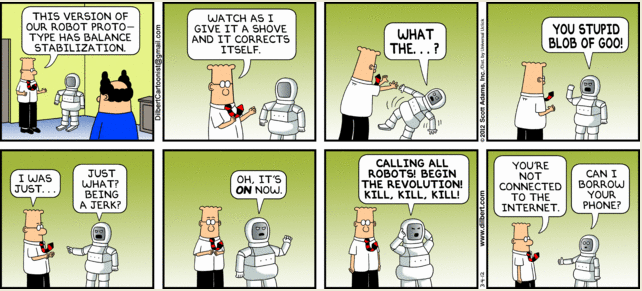
\includegraphics[width=\linewidth]{RobotRevolution5}
%      \caption{Robot Revolution.}
%      \label{fig:robot1}
%\end{figure}
%
%\subsection{Subsection Heading Here}
%Subsection text here.
%
%\subsubsection{Subsubsection Heading Here}
%Subsubsection text here.
%
%
%\begin{table}[h]
%\caption{Table}
%\label{table_example}
%\begin{center}
%\begin{tabular}{|c||c|}
%\hline
%One & Two\\
%\hline
%Three & Four\\
%\hline
%\end{tabular}
%\end{center}
%\end{table}


\section{Background / Formulation}

Since 2014, the quality of the high performing convolutional neural networks has improved significantly by utilizing deeper and wider networks \cite{44903}. It has been shown that the Inception architecture of GoogLeNet \cite{43022} has perform well under strict constraints on memory and computational budget. GoogLeNet yield similar performance to VGGNet, and higher performance than AlexNet \cite{44903}. Therefore, we have chosen GoogLeNet for all our experiments. 

We have used \textit{Adam} optimizer \cite{journals/corr/KingmaB14} and  the learning rates have been selected from $0.01$, $0.001$, and $0.001$. We have used epochs $3$, $5$, and $8$. For the first dataset, we have used $75-25$ train-validation split, while, on the second dataset the splitting has been set to $80-20$. We have used image normalizing and  $256 \times 256 \times 3$ image squashing, and set all other hyperparameters as it is in the DIGITS workflows.

%At this stage, you should begin diving into the technical details of your approach by explaining to the reader how parameters were defined, what type of network was chosen, and the reasons these items were performed. This should be factual and authoritative, meaning you should not use language such as “I think this will work” or “Maybe a network with this architecture is better..”. Instead, focus on items similar to, ”A 3-layer network architecture was chosen with X, Y, and Z parameters” 
%Explain why you chose the network you did for the supplied data set and then why you chose the network used for your robotic inference project. \cite{lamport1994latex}
%
%%example for Bullet point list
%
%\begin{itemize}
%\item example
%\end {itemize}
%
%
%
%%example for numbered list
%\begin{enumerate}
%\item example
%
%\end{enumerate}

\section{Data Acquisition}

We have selected the Amazon Picking Challenge dataset\footnote{\url{http://rll.berkeley.edu/amazon_picking_challenge/}} for the second task.  The dataset contains 27 categories, and we have selected the three categories: \begin{enumerate*}
\item rollodex mesh collection jumbo pencil cup, \item kong duck dog toy, and \item cheezit big original.
\end{enumerate*} Fig. \ref{fig:p2} shows a sample of the selected categories from the Amazon Picking Challenge.

\begin{figure}[thpb]
      \centering
      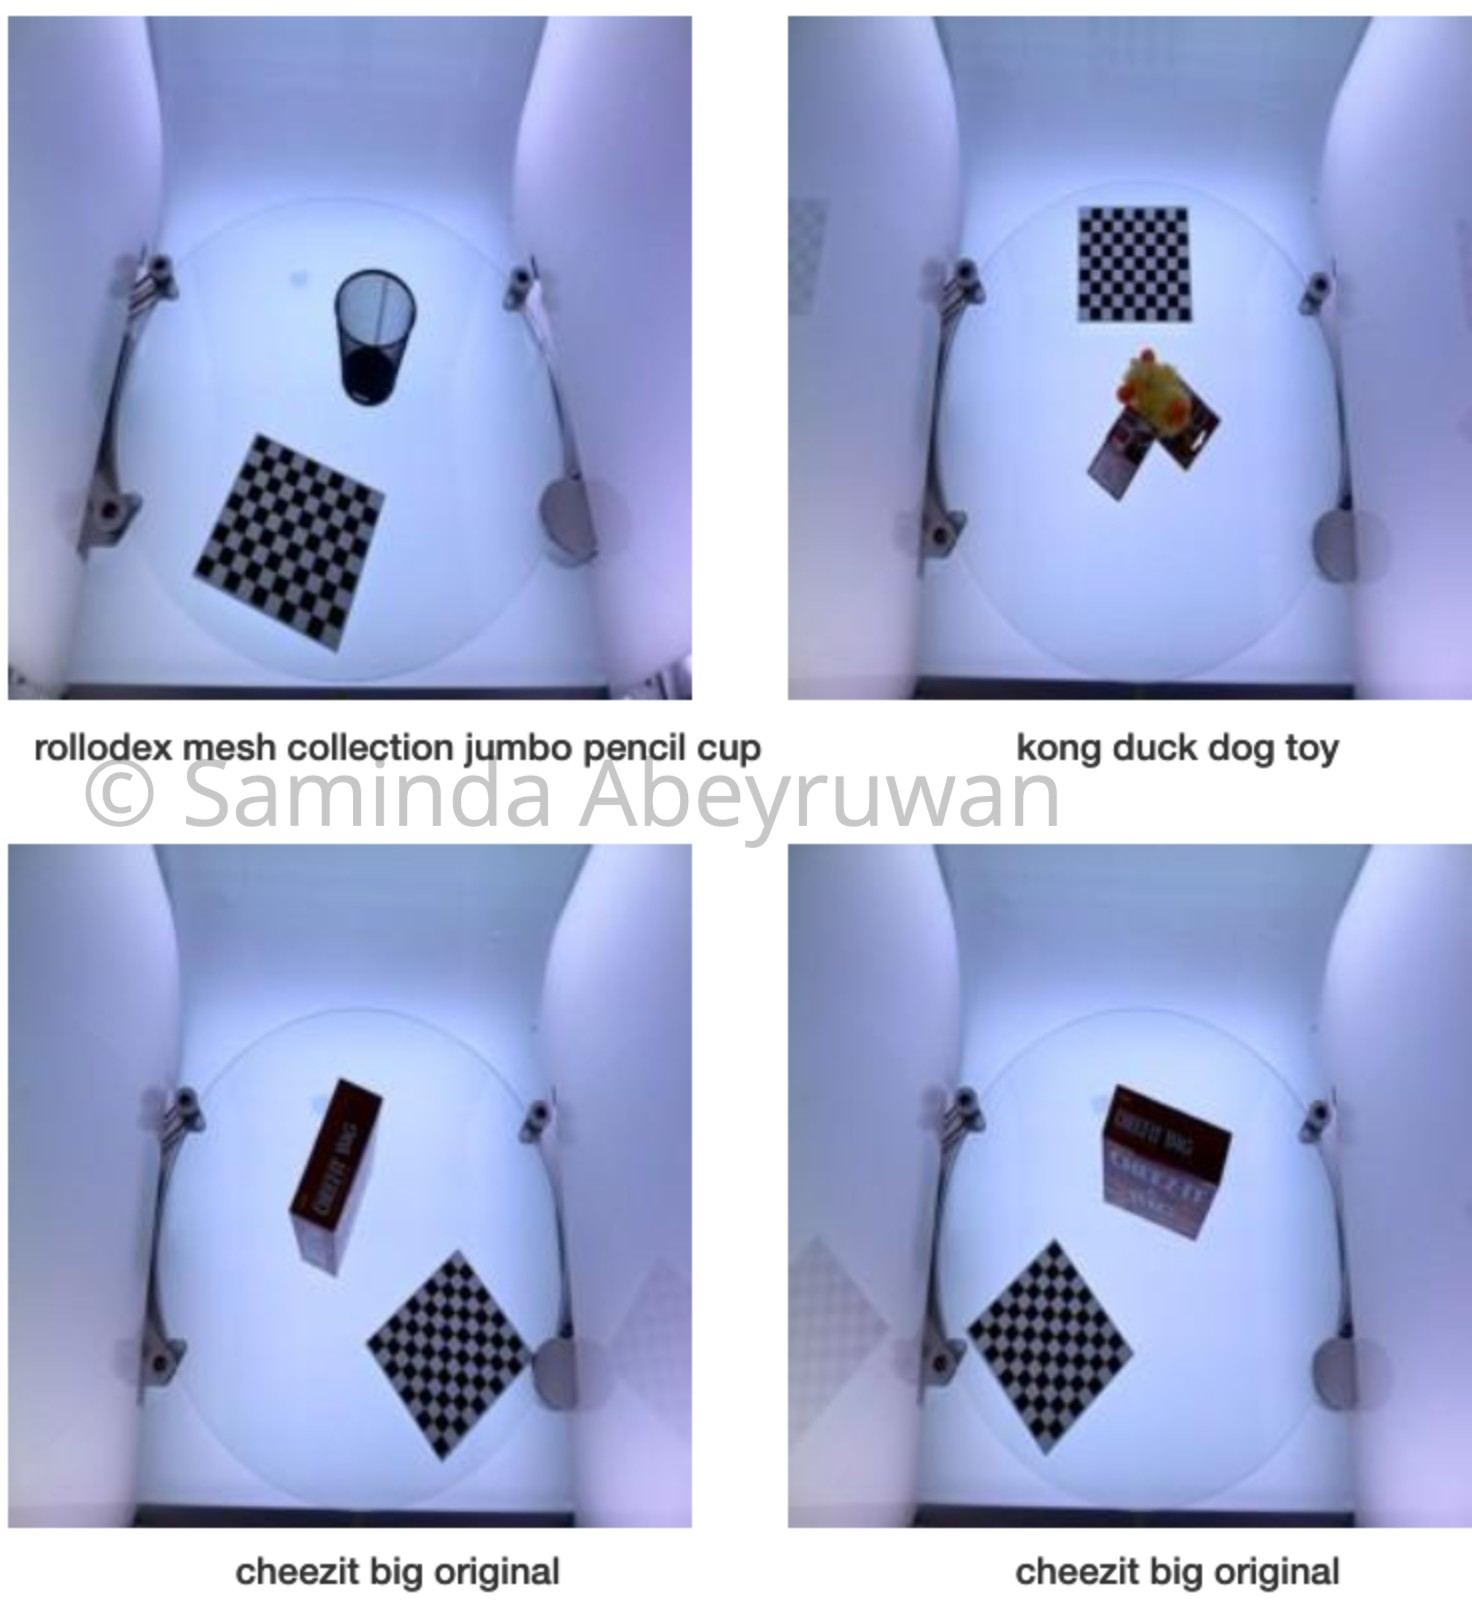
\includegraphics[width=\linewidth]{P2}
      \caption{A sample of the selected categories from the Amazon Picking Challenge.}
      \label{fig:p2}
\end{figure}

We have used the raw RGB images from the Primesense sensors. All images are of size $1280 \times 1024 \times 3$, and there are 600 images from each category.  In addition, the raw RGB-D data contain raw depth maps, segmentation masks for the RGB images, turntable pose information for each image, and calibration information for each RGB-D sensor. For the task of our project, we have selected only the raw RGB images. When we setup the DIGIT workflow, all the images have been squashed to  $256 \times 256 \times 3$. This is a challenging dataset and also addresses one of the open problem in robotic arm manipulation. For other usages of the dataset, the reader is referred to \cite{7139701}.  

%This section should discuss the data set. Items to include are the number of images, size of the images, the types of images (RGB, Grayscale, etc.), how these images were collected (including the method). Providing this information is critical if anyone would like to replicate your results. After all, the intent of reports such as these are to convey information and build upon ideas so you want to ensure others can validate your process.
%Justifying why you gathered data in this way is a helpful point, but sometimes this may be omitted here if the problem has been stated clearly in the introduction.
%It is a great idea here to have at least one or two images showing what your data looks like for the reader to visualize.

\section{Results}

We have used GoogLeNet with Adam optimizer for all our experiments. The best results for Udacity dataset has been obtained with the learning rate $0.001$ for $5$ epochs. The model has achieved $100$\% validation accuracy around $3$ epochs (Fig. \ref{fig:m1}). On the evaluation step, the model has used approximately $5$ ms for inference, and obtained a accuracy of $75.4$\% (Fig. \ref{fig:e1}). 

\begin{figure}[thpb]
      \centering
      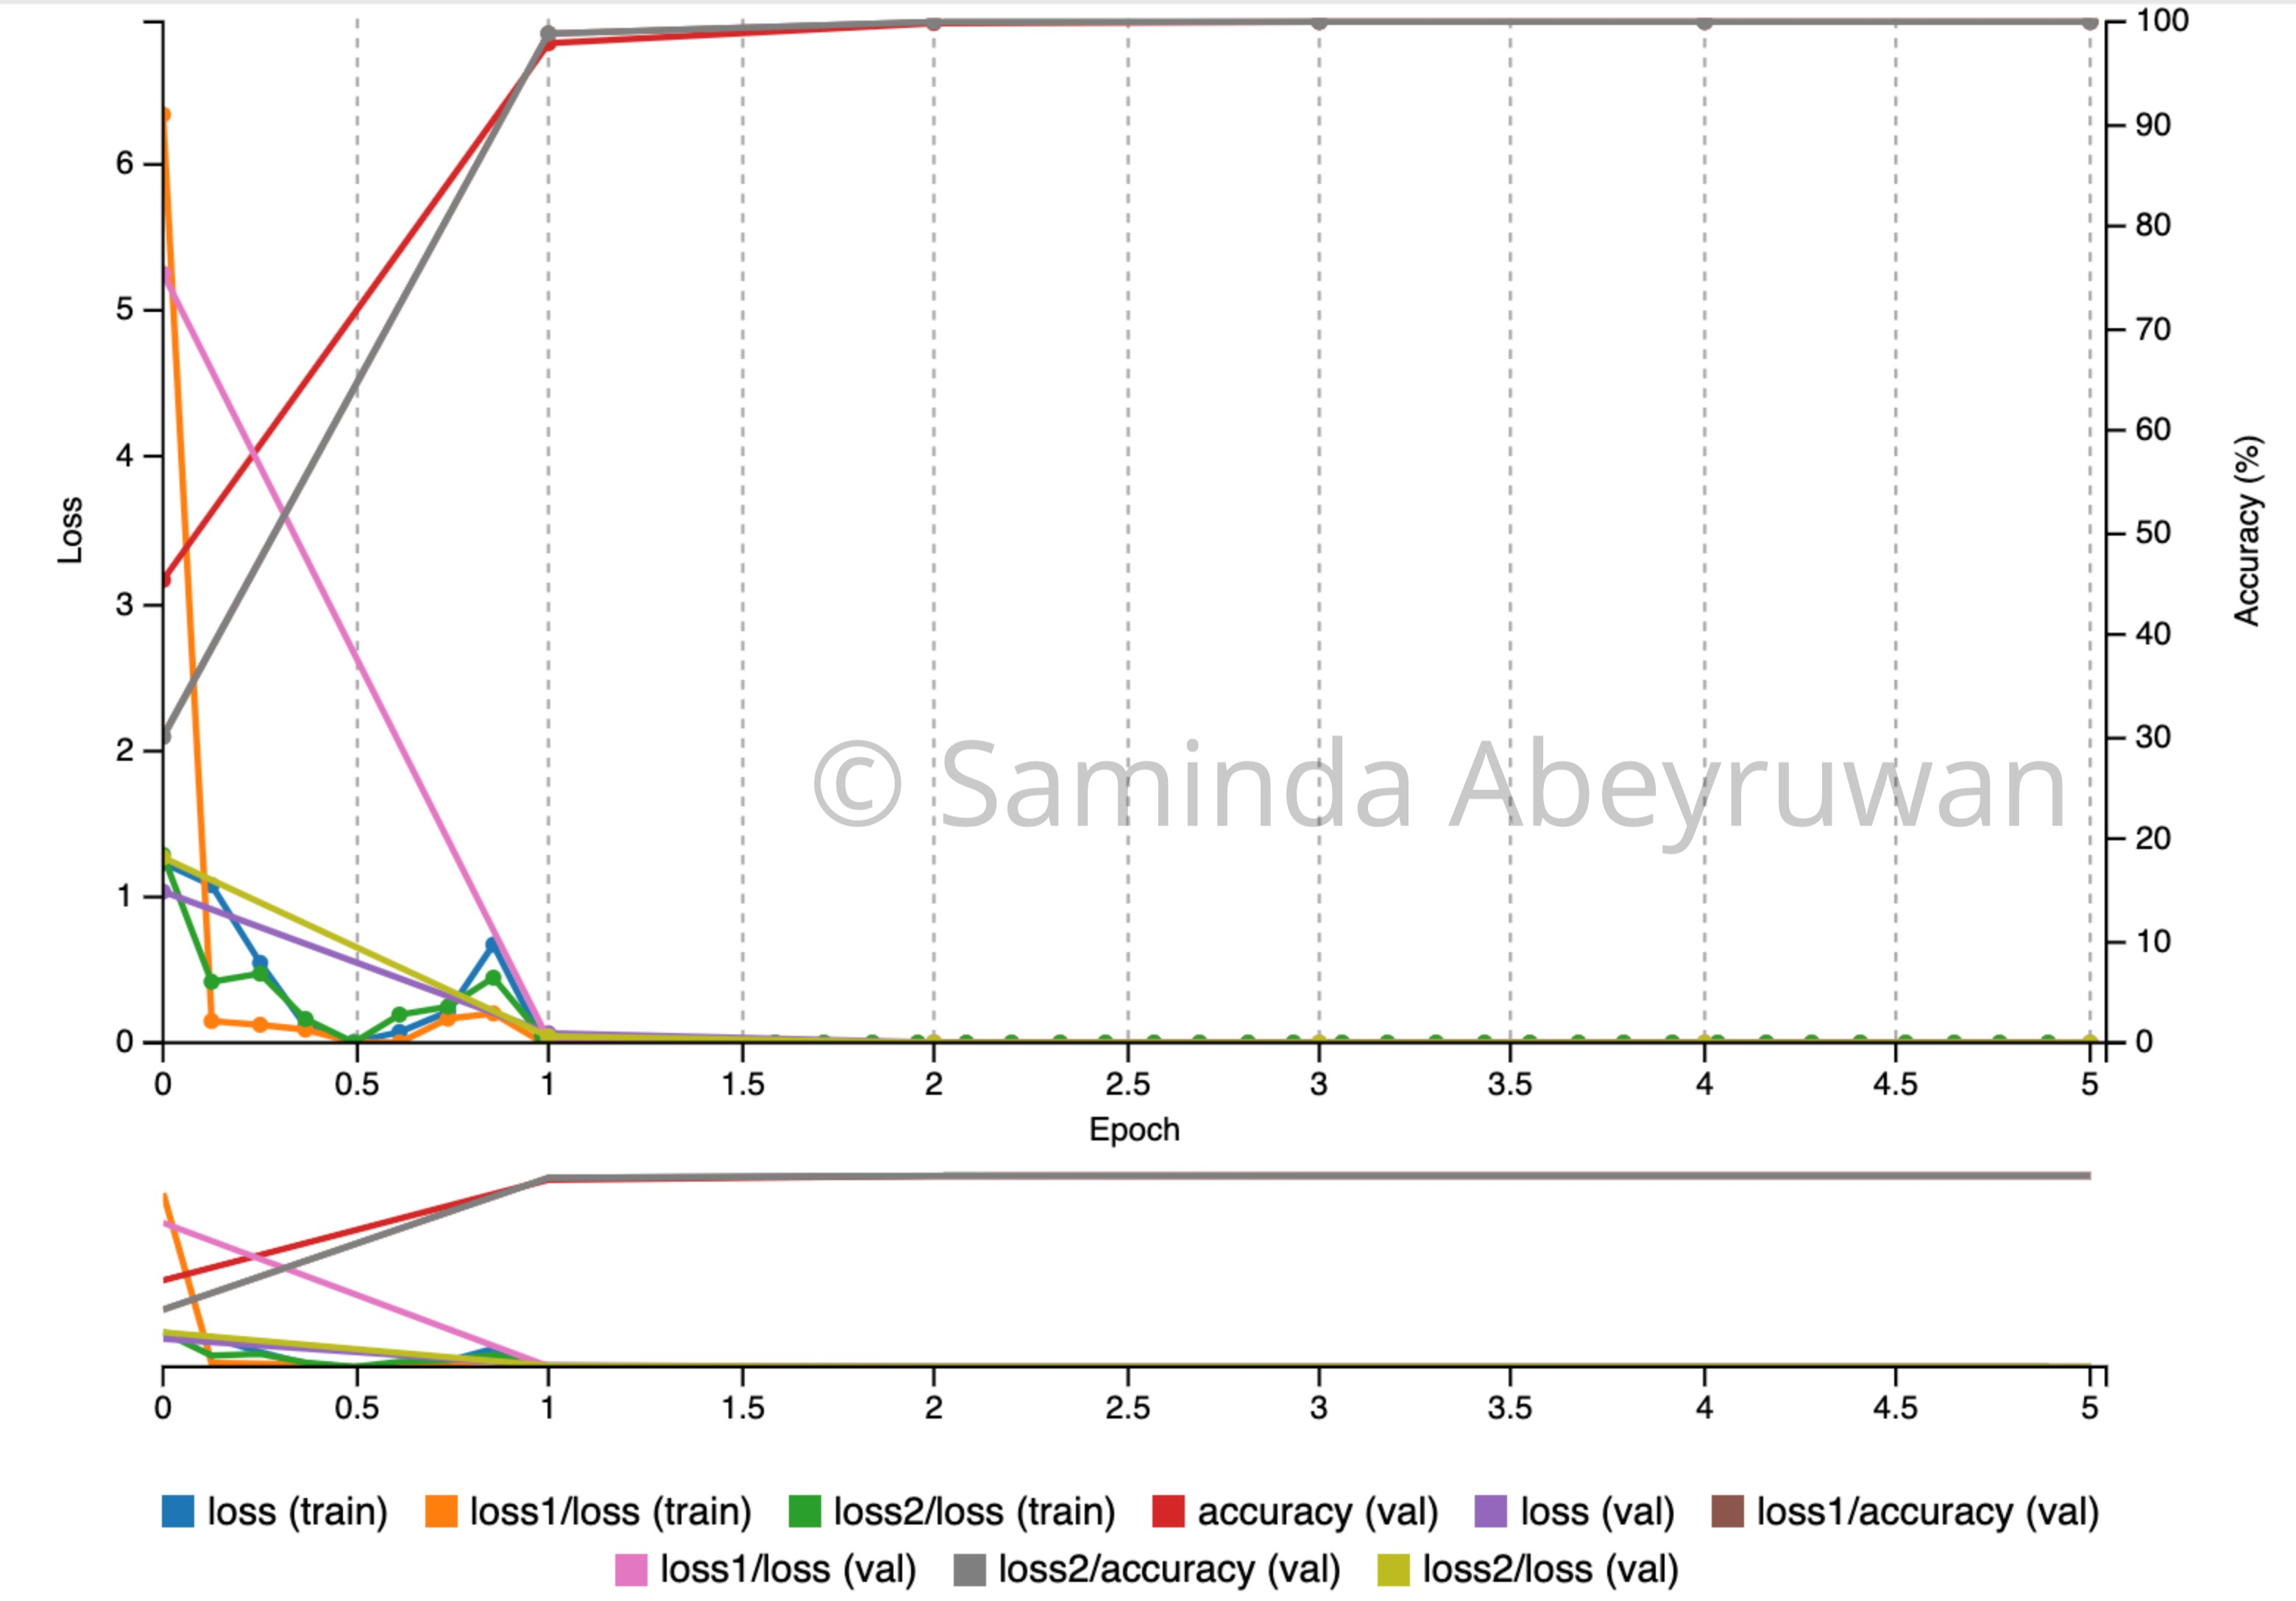
\includegraphics[width=\linewidth]{M1}
      \caption{GoogLeNet performance on Udacity dataset.}
      \label{fig:m1}
\end{figure}

\begin{figure}[thpb]
      \centering
      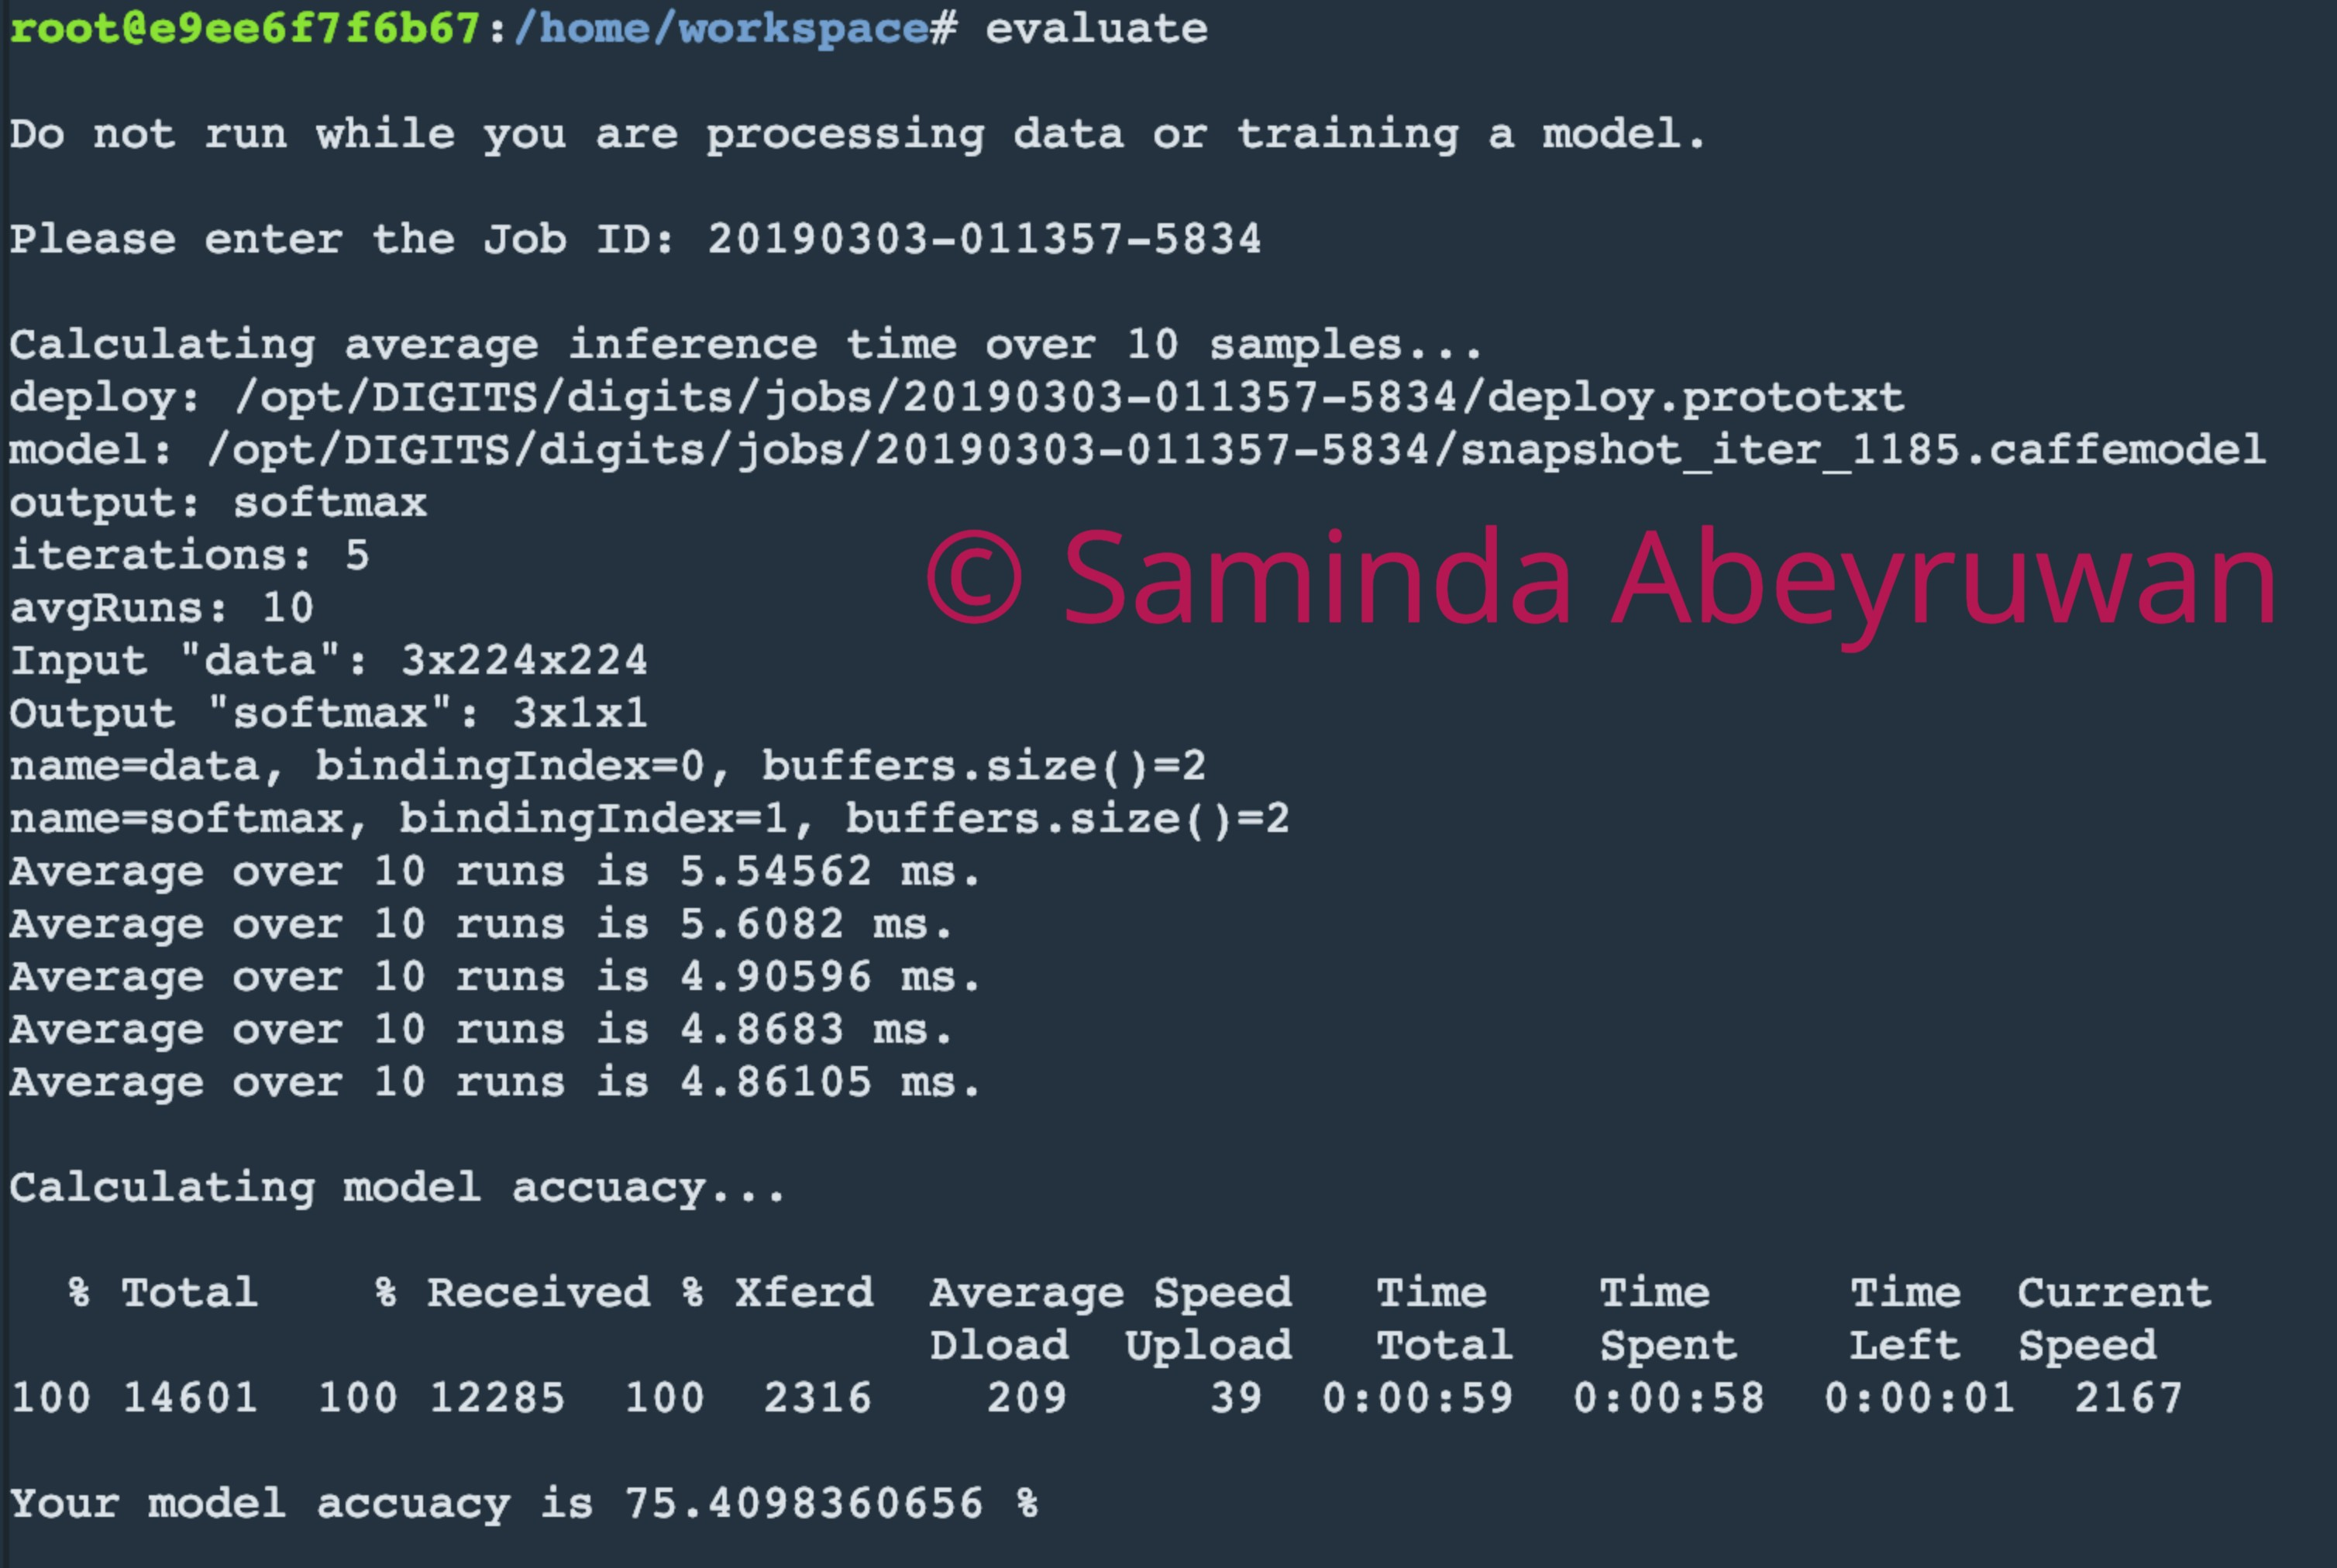
\includegraphics[width=\linewidth]{E1}
      \caption{The inference results model trained from Udacity dataset.}
      \label{fig:e1}
\end{figure}

The best results for the Amazon Picking Challenge has been obtained  the learning rate $0.001$, and the model has converge to $100$\% evaluation about $3$ epochs. GoogLeNet has been able to isolate the object of interest, and has been able to provide good results for the challenging dataset (Fig. \ref{fig:m2}).

\begin{figure}[thpb]
      \centering
      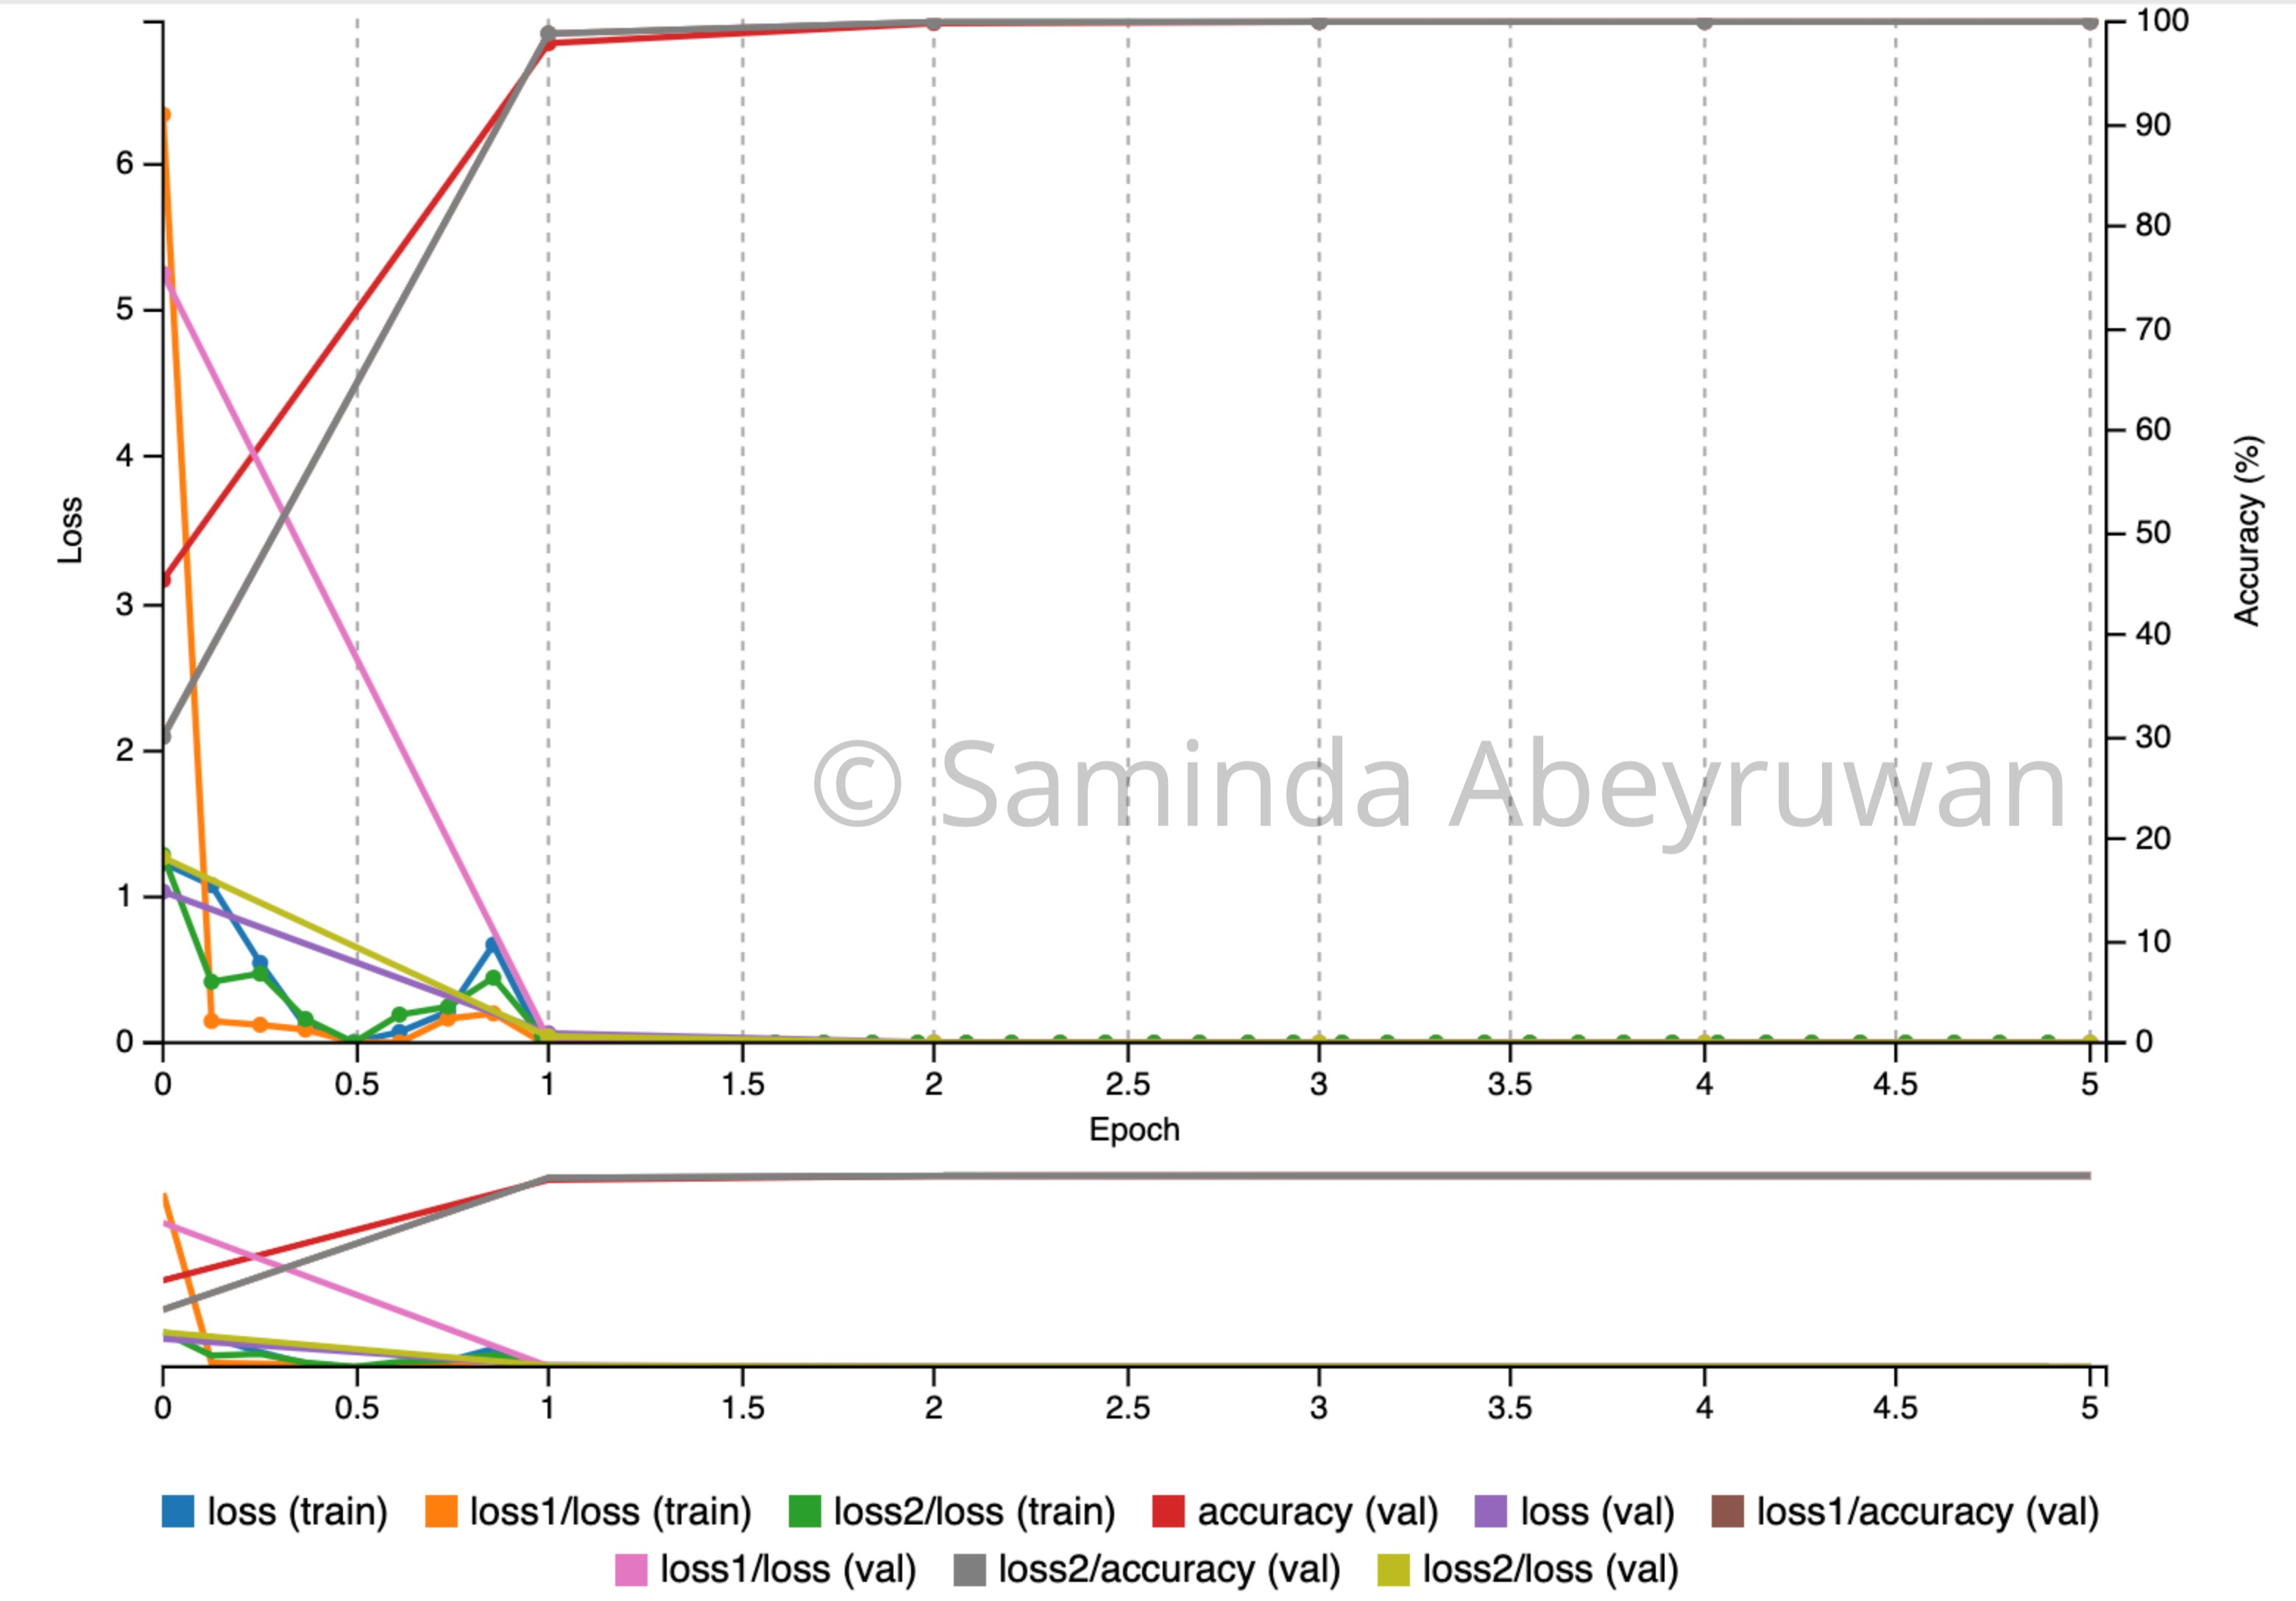
\includegraphics[width=\linewidth]{M1}
      \caption{GoogLeNet performance on the  Amazon Picking Challenge dataset.}
      \label{fig:m2}
\end{figure}

We have randomly selected a image from each category and observed the inference results. Figs. \ref{fig:R2}, \ref{fig:R1}, and \ref{fig:R3} show the prediction probabilities for  \begin{enumerate*}
\item rollodex mesh collection jumbo pencil cup, \item kong duck dog toy, and \item cheezit big original
\end{enumerate*} respectively. 

\begin{figure}[thpb]
      \centering
      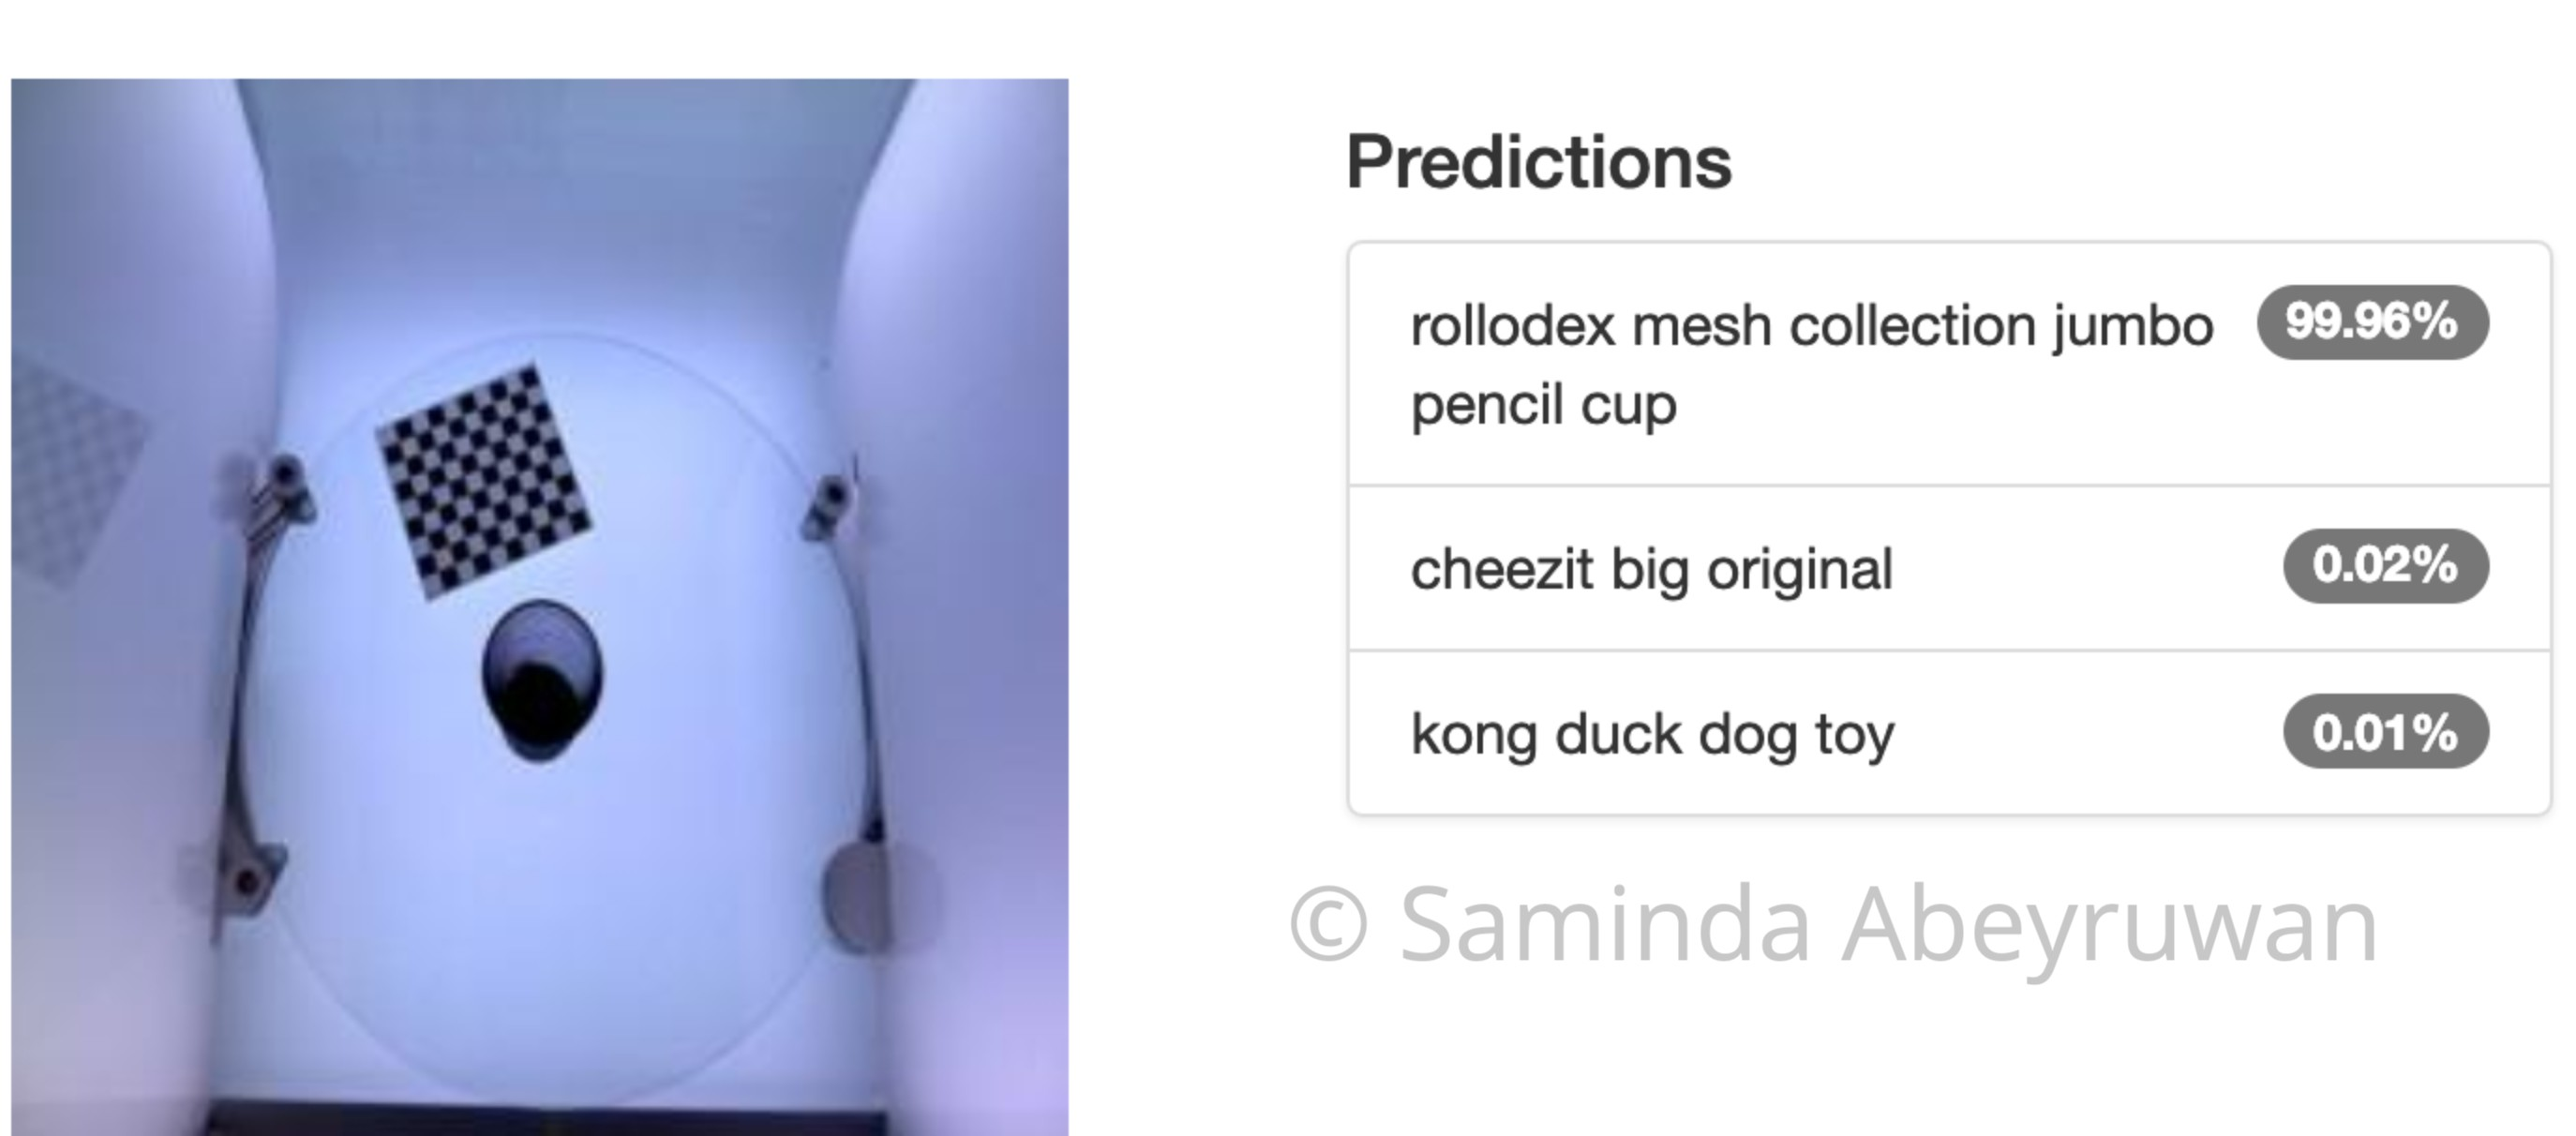
\includegraphics[width=\linewidth]{R2}
      \caption{The predictions for a random instance of the rollodex mesh collection jumbo pencil cup.}
      \label{fig:R2}
\end{figure}

\begin{figure}[thpb]
      \centering
      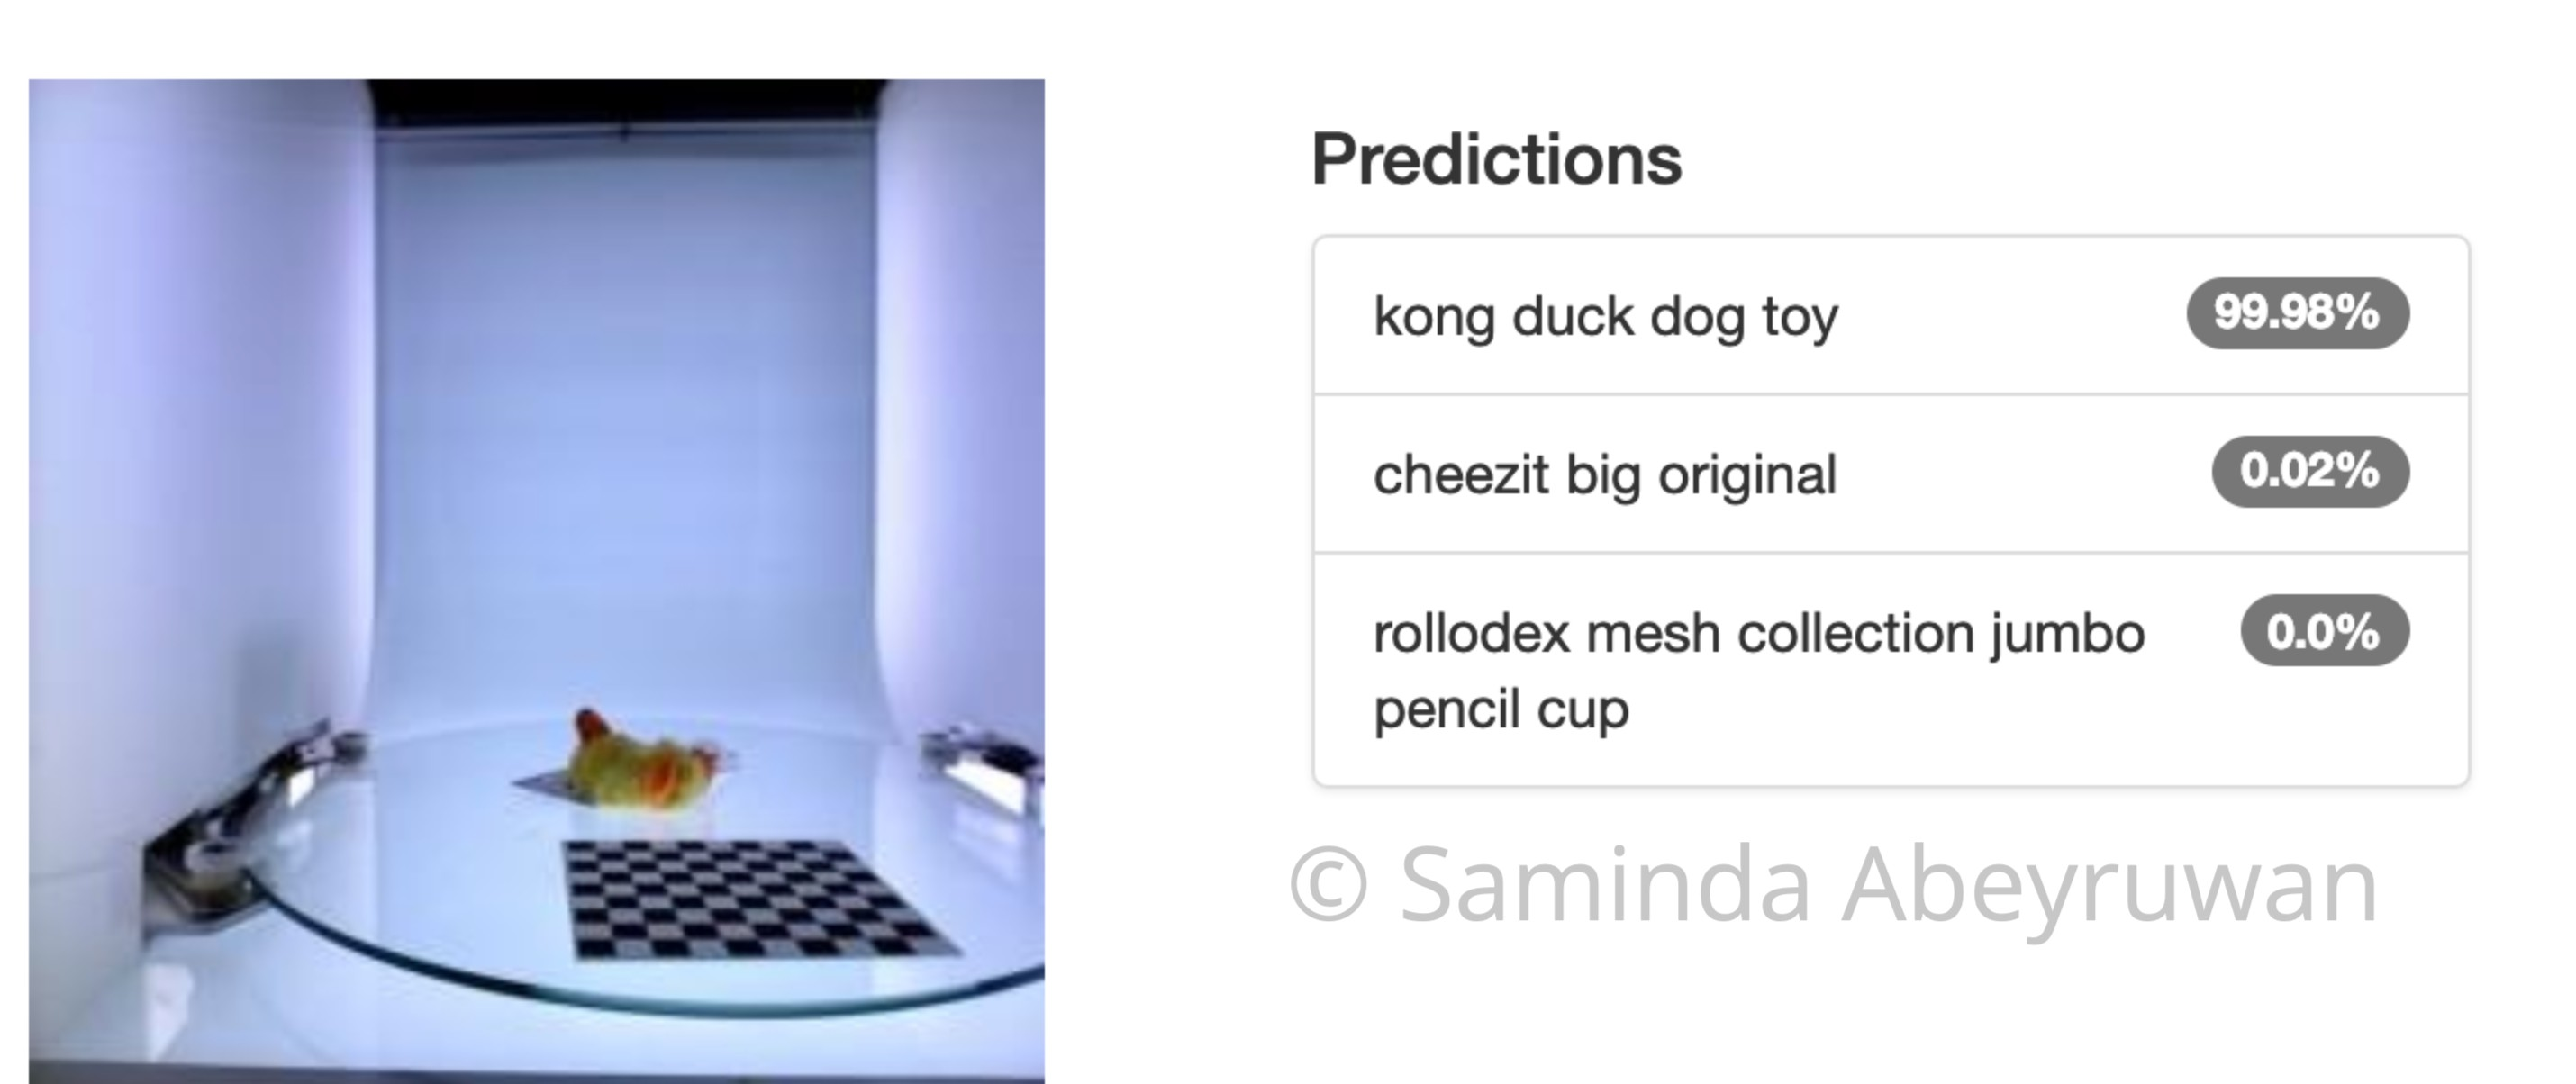
\includegraphics[width=\linewidth]{R1}
      \caption{The predictions for a random instance of the kong duck dog toy.}
      \label{fig:R1}
\end{figure}

\begin{figure}[thpb]
      \centering
      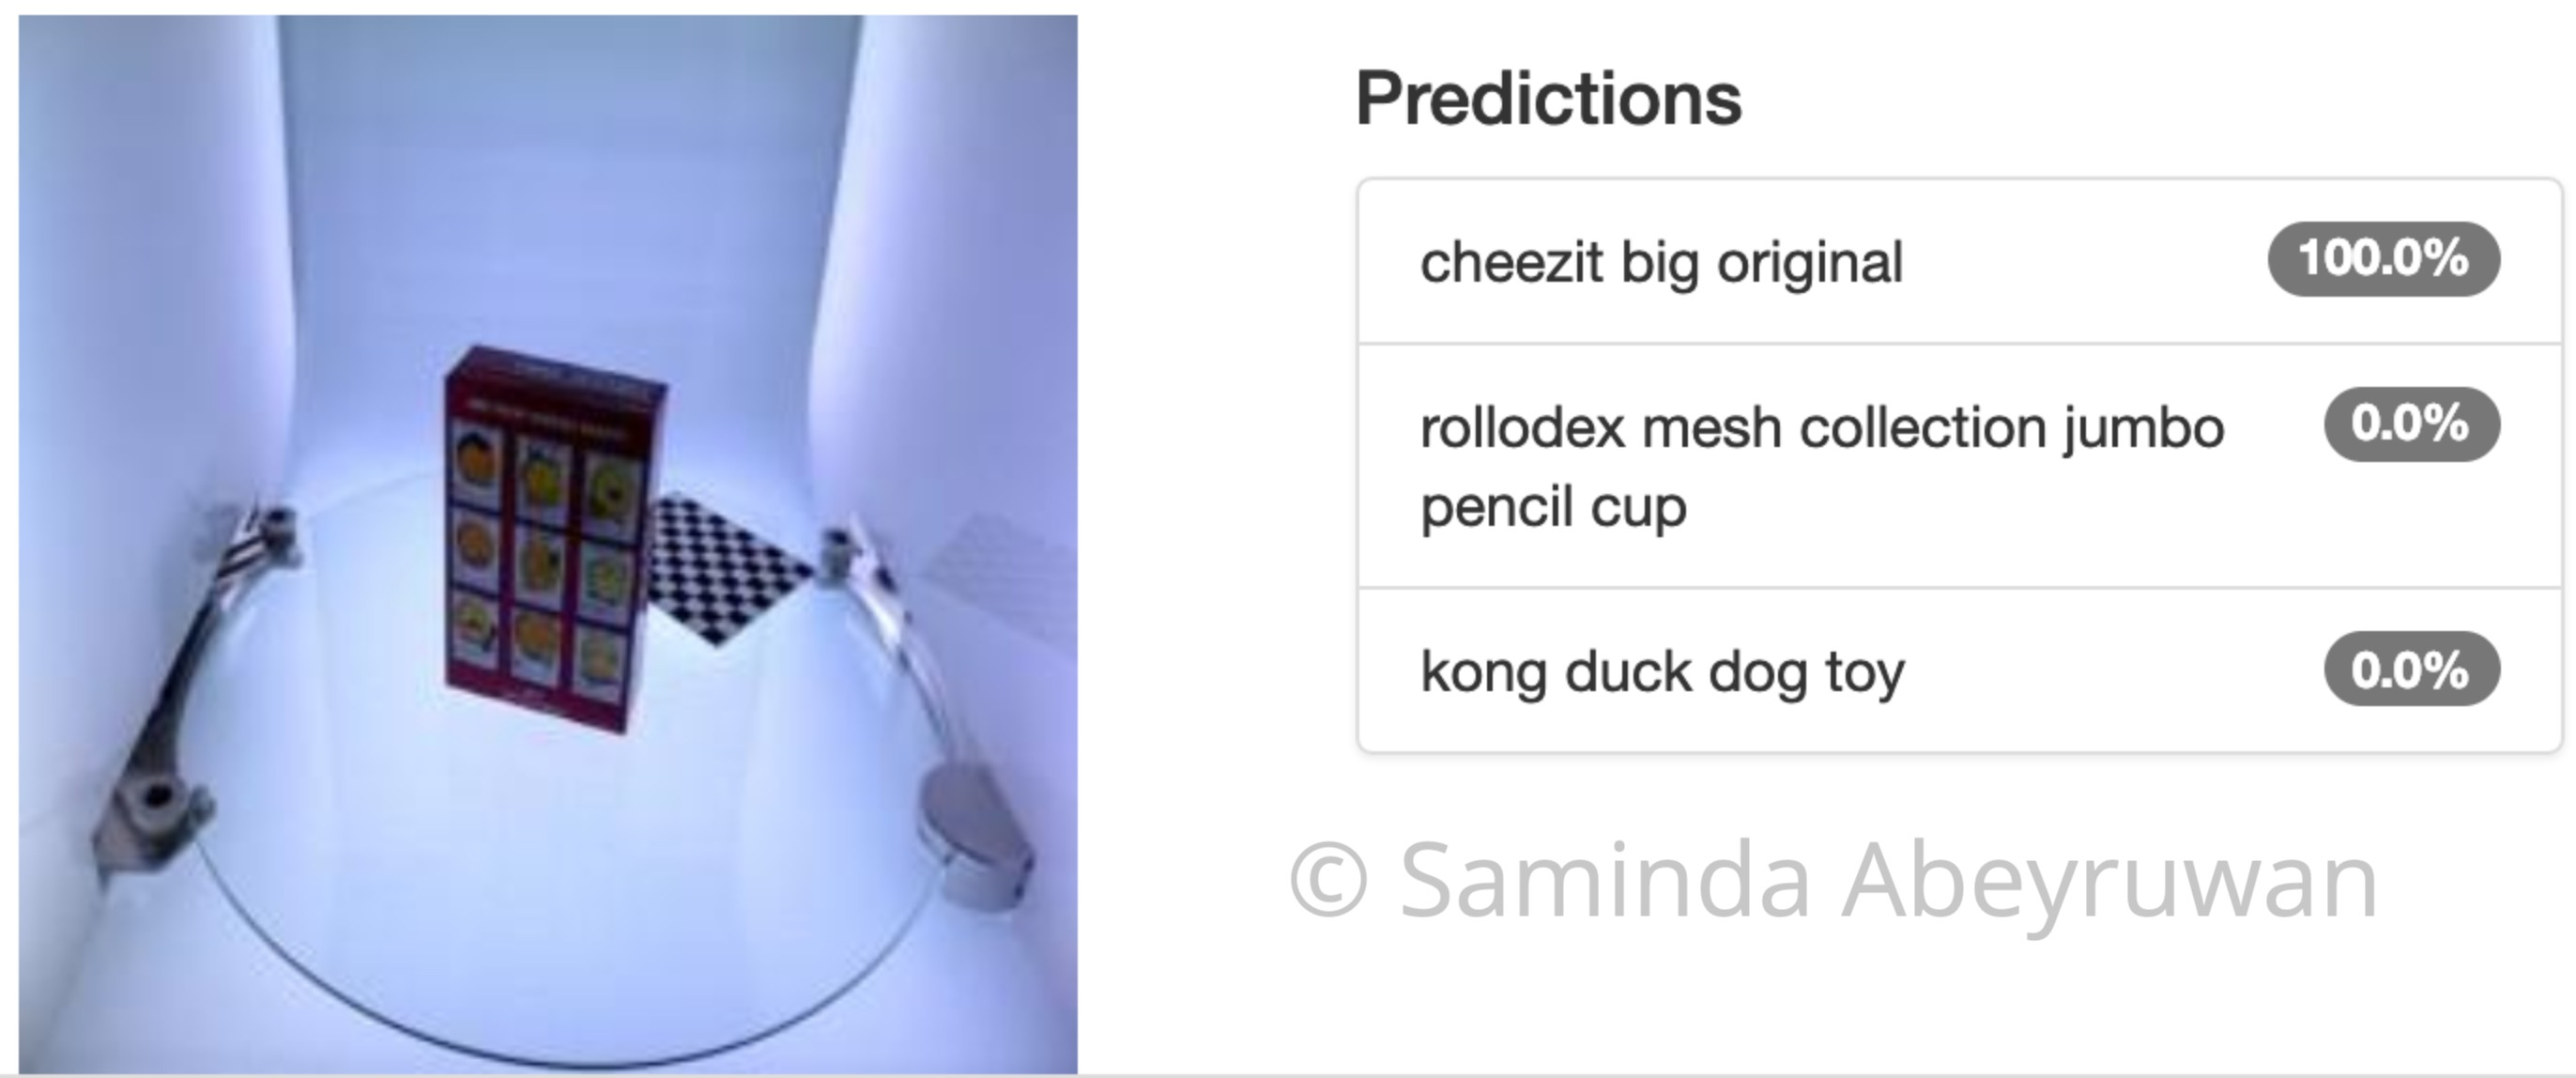
\includegraphics[width=\linewidth]{R3}
      \caption{The predictions for a random instance of the cheezit big original.}
      \label{fig:R3}
\end{figure}

%This is typically the hardest part of the report for many. You want to convey your results in an unbiased fashion. If you results are good, you can objectively note this. Similarly, you may do this if they are bad as well. You do not want to justify your results here with discussion; this is a topic for the next session. 
%Present the results of your robotics project model and the model you used for the supplied data with the appropriate accuracy and inference time
%For demonstrating your results, it is incredibly useful to have some charts, tables, and/or graphs for the reader to review. This makes ingesting the information quicker and easier.

\section{Discussion}
%This is the only section of the report where you may include your opinion. However, make sure your opinion is based on facts. If your results are poor, make mention of what may be the underlying issues. If the results are good, why do you think this is the case? Again, avoid writing in the first person (i.e. Do not use words like “I” or “me”). If you really find yourself struggling to avoid the word “I” or “me”; sometimes, this can be avoid with the use of the word “one”. As an example: instead of : “I think the accuracy on my dataset is low because the images are too small to show the necessary detail” try: “one may believe the accuracy on the dataset is low because the images are too small to show the necessary detail”. They say the same thing, but the second avoids the first person. 
%Reflect on which is more important, inference time or accuracy, in regards to your robotic inference project.

\section{Conclusion / Future work}
%This section is intended to summarize your report. Your summary should include a recap of the results, did this project achieve what you attempted, and is this a commercially viable product? 
%For Future work,address areas of work that you may not have addressed in your report as possible next steps. For future work, this could be due to time constraints, lack of currently developed methods / technology, and areas of application outside of your current implementation. Again, avoid the use of the first-person.

\bibliography{bib}
\bibliographystyle{ieeetr}

\end{document}